% % % % % % % % % % % % % % % % % % % % % % % % % % % % % % % % % %
%  Devolutiva — Fase 1: Imersão
%  Disciplina: Design Thinking (DE_233) — ETE Cícero Dias
%  Profa. Samara Silva  ·  Recife, 19 de junho de 2026
% % % % % % % % % % % % % % % % % % % % % % % % % % % % % % % % % %

\documentclass[
  sigconf,
  nonacm, % Remove o rodapé da ACM
  language=portuguese
]{acmart}

% ── Desliga rodapé ACM ──────────────────────────────────────
\settopmatter{printacmref=false}
\setcopyright{none}
\acmYear{2026}
\let\balance\relax

% ── Mata a página temporária da ACM (compilação única via API) ──
\makeatletter
\def\acm@addtemp@page{}
\makeatother

% ── Pacotes ─────────────────────────────────────────────────
\usepackage[portuguese]{babel}
\usepackage{microtype}
\usepackage{booktabs}
\usepackage{tabularx}
\usepackage{array}
\usepackage{colortbl}
\usepackage[dvipsnames,table]{xcolor}
\usepackage[inline]{enumitem}
\usepackage{graphicx}
\usepackage{adjustbox}
\usepackage{fancyhdr}
\usepackage{eso-pic} % Para a capa preencher toda a página sem gerar páginas em branco

% ── Ajuste contra quebras de texto ruins (Textos Cortados) ──
\tolerance=1000
\emergencystretch=1.5em

% ── Cores ───────────────────────────────────────────────────
\definecolor{cgood}{HTML}{1E6B3A}
\definecolor{cwarn}{HTML}{8B4500}
\definecolor{cred}{HTML}{C0392B}
\definecolor{cmuted}{HTML}{666666}
\definecolor{crow}{HTML}{F2EFEB}

% ── Colunas customizadas para tabela ────────────────────────
\newcolumntype{L}[1]{>{\raggedright\arraybackslash}p{#1}}
\newcolumntype{C}[1]{>{\centering\arraybackslash}p{#1}}

% ── Comando nota destacada ───────────────────────────────────
\newcommand{\notadestaque}[2]{%
  \noindent\textbf{Nota:}\enspace%
  {\large\bfseries\color{cred}#1\,/\,#2\,pts}%
}

% ── Comando label de status ──────────────────────────────────
\newcommand{\statusok}[1]{{\small\bfseries\color{cgood}#1}}
\newcommand{\statuswarn}[1]{{\small\bfseries\color{cwarn}#1}}

% ── Renomeações PT-BR ────────────────────────────────────────
\AtBeginDocument{%
  \renewcommand{\abstractname}{Resumo}
  \renewcommand{\figurename}{Figura}
  \renewcommand{\tablename}{Tabela}
}

% ────────────────────────────────────────────────────────────
\begin{document}

% ── CAPA ────────────────────────────────────────────────────
\thispagestyle{empty}
\AddToShipoutPictureBG*{%
  \AtPageLowerLeft{%
    \IfFileExists{capa.png}{%
      
\includegraphics[width=\paperwidth,height=\paperheight]{capa.png}%
    }{%
      \IfFileExists{../../capa.png}{%
        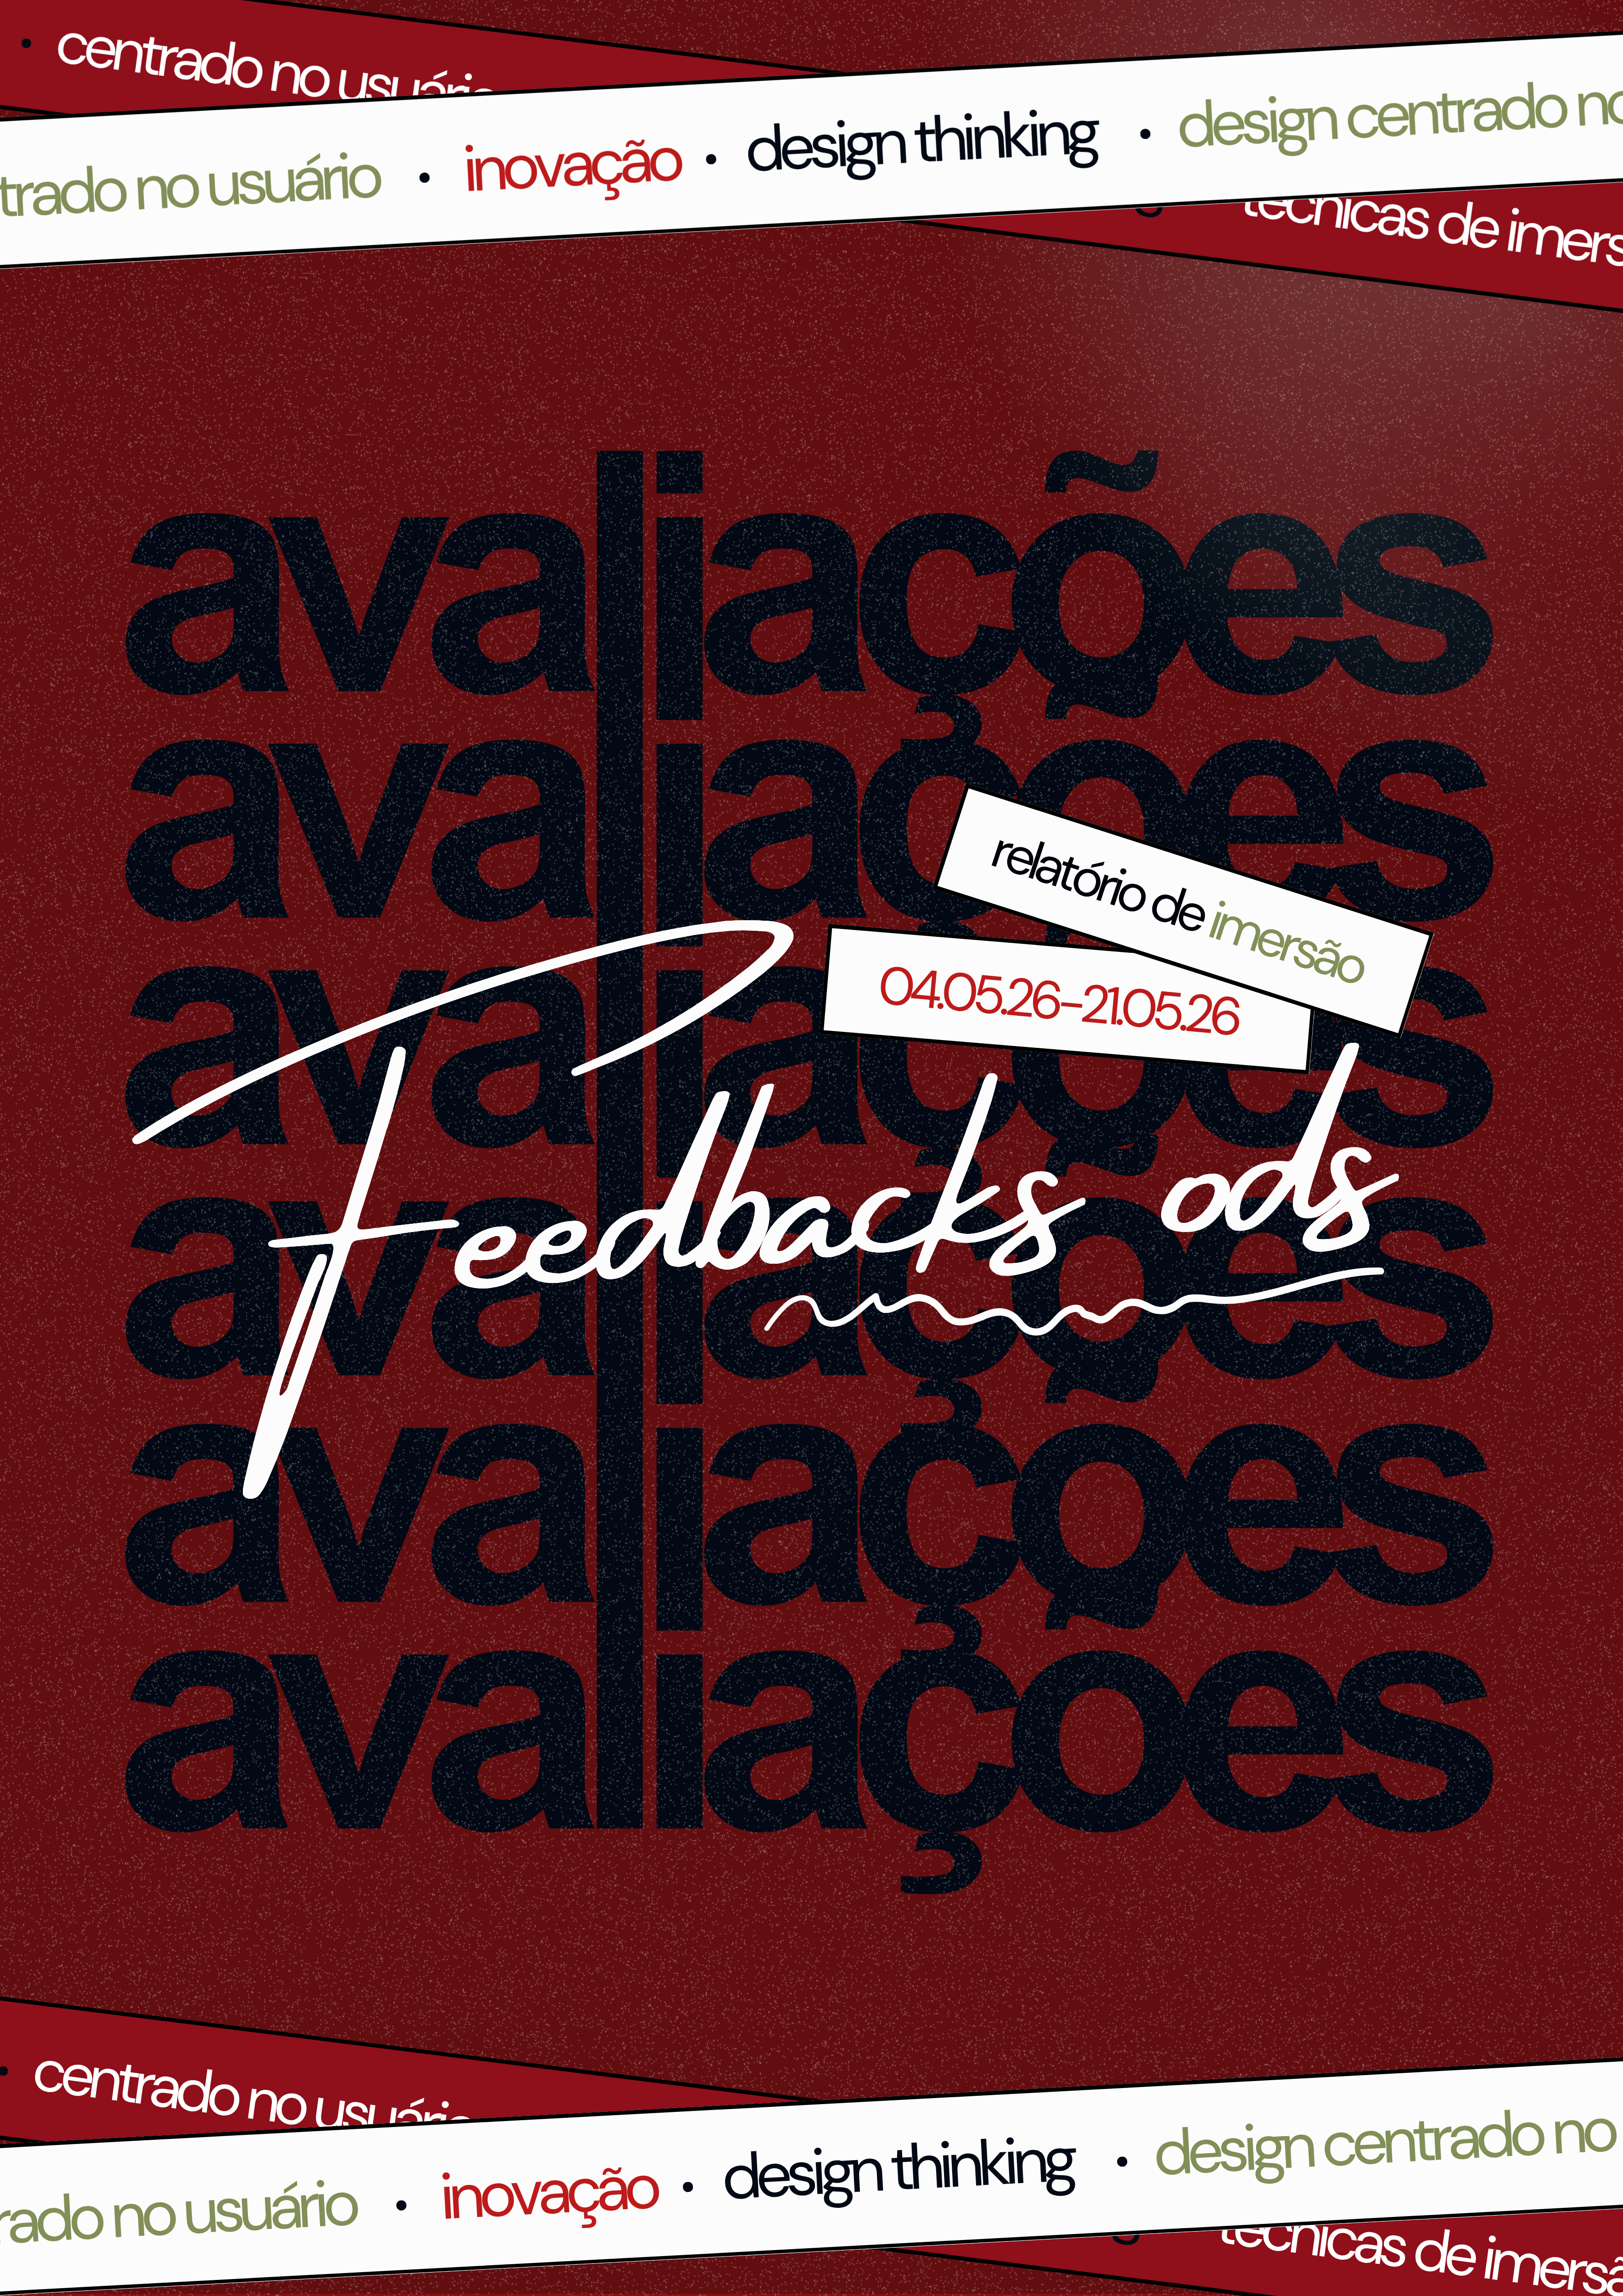
\includegraphics[width=\paperwidth,height=\paperheight]{../../capa.png}%
      }{%
        \parbox[b][\paperheight]{\paperwidth}{%
          \vspace*{10cm}\begin{center}{\large\color{gray}[capa.png não encontrada]}\end{center}%
        }%
      }%
    }%
  }%
}
\mbox{} % Caixa vazia para garantir que a página da capa seja gerada e preenchida
\clearpage

% ── CONFIGURAÇÃO DE PÁGINA PÓS-CAPA ─────────────────────────
\setcounter{page}{1}
\pagestyle{fancy}
\fancyhf{}
\renewcommand{\headrulewidth}{0pt}
\fancyfoot[C]{\thepage}
\setlength{\headsep}{0.8cm} % Distancia o cabeçalho do conteúdo das colunas

% ── METADADOS ────────────────────────────────────────────────
\title{Feedback Avaliativo de Projeto: Design Thinking --- Fase 2 — Definição}

\author{Profa.\ Samara Silva}
\authornote{Grupo: \textbf{Grupo 01 - Fome Zero} \textperiodcentered\ Per\'{i}odo: 22 de maio de 2026 \textperiodcentered\ Avaliado em: 19 de junho de 2026.}
\email{samarasilvia.educa@gmail.com}
\affiliation{%
  \institution{ETE C\'{i}cero Dias}
  \department{M\'{o}dulo 1 --- Turma A · 2026.1}
  \city{Recife}
  \state{Pernambuco}
  \country{Brasil}
}

\author{Grupo 01 - Fome Zero}
\affiliation{%
  \institution{ETE C\'{i}cero Dias}
  \department{Turma --- Turma A · 2026.1}
  \city{Recife}
  \state{Pernambuco}
  \country{Brasil}
}
\maketitle

\vspace{1em}
\section{Avaliação Geral}

\notadestaque{2,60}{3,00}

A avaliação foi concluída. A seguir o resumo dos critérios e os comentários detalhados.

\subsection{Resumo dos Critérios}

\rowcolors{2}{crow}{white}
\begin{tabular}{@{} L{2.6cm} C{2.5cm} C{1.1cm} C{1.1cm} @{}}
\toprule
\textbf{Critério} & \textbf{Status} & \textbf{Nota} & \textbf{Máx.} \\
\midrule
Persona com Empatia Real & \statuswarn{Completo c/ ressalvas} & \textbf{0,42} & 0,50 \\
Mapa de Empatia como Ferramenta & \statuswarn{Completo c/ ressalvas} & \textbf{0,85} & 1,00 \\
Enunciado do Problema & \statusok{Completo} & \textbf{1,00} & 1,00 \\
Jornada do Usuário (ASTOIS) & \statuswarn{Faltou pouco} & \textbf{0,33} & 0,50 \\
\midrule
\textbf{Total} & & \textbf{\color{cred}2,60} & \textbf{3,00} \\
\bottomrule
\end{tabular}

\section{Comentários por Critério}

\subsection{Persona com Empatia Real}

\noindent\statuswarn{0,42\,/\,0,50 pts · Completo c/ ressalvas}

\begin{itemize}[leftmargin=14pt,itemsep=1pt,topsep=3pt,parsep=0pt]
  \item[\textcolor{cgood}{$\checkmark$}] {\small\textcolor{cgood}{Nome próprio que humaniza o arquétipo}}
  \item[\textcolor{cgood}{$\checkmark$}] {\small\textcolor{cgood}{Representação visual coerente (foto/avatar)}}
  \item[\textcolor{cgood}{$\checkmark$}] {\small\textcolor{cgood}{Papel/arquétipo-síntese (o rótulo: ex: "Pequeno Comerciante")}}
  \item[\textcolor{cgood}{$\checkmark$}] {\small\textcolor{cgood}{Dados demográficos (idade, gênero, localização, escolaridade, ocupação, estado civil)}}
  \item[\textcolor{cgood}{$\checkmark$}] {\small\textcolor{cgood}{Contexto/bio que situa a vida da pessoa}}
  \item[$\square$] {\small\textcolor{cmuted}{Características de personalidade (traços comportamentais)}}
  \item[\textcolor{cgood}{$\checkmark$}] {\small\textcolor{cgood}{Motivação (o que move)}}
  \item[$\square$] {\small\textcolor{cmuted}{Objetivos/metas}}
  \item[\textcolor{cgood}{$\checkmark$}] {\small\textcolor{cgood}{Dores/frustrações}}
  \item[\textcolor{cgood}{$\checkmark$}] {\small\textcolor{cgood}{Citação-síntese que captura a essência}}
  \item[\textcolor{cgood}{$\checkmark$}] {\small\textcolor{cgood}{Ancoragem na imersão — a persona é síntese da pesquisa de campo, não invenção/suposição}}
  \item[\textcolor{cgood}{$\checkmark$}] {\small\textcolor{cgood}{Arquétipo comportamental, não estereótipo ou caricatura}}
  \item[\textcolor{cgood}{$\checkmark$}] {\small\textcolor{cgood}{Coerência interna — motivação → objetivos → dores se sustentam mutuamente}}
  \item[\textcolor{cgood}{$\checkmark$}] {\small\textcolor{cgood}{Conexão com o problema e o ODS do projeto}}
  \item[\textcolor{cgood}{$\checkmark$}] {\small\textcolor{cgood}{Especificidade — detalhes concretos que humanizam vs. genérico ("homem de 40 anos qualquer")}}
  \item[\textcolor{cgood}{$\checkmark$}] {\small\textcolor{cgood}{Define claramente as tarefas críticas que o usuário precisa executar}}
\end{itemize}

\textbf{Impressões antes de ler o relatório}

Com base na leitura da persona e na releitura do primeiro relatório, observa-se que a persona está bem estruturada e coerente com os dados coletados. No entanto, surge uma dúvida em relação à matriz de alinhamento, na qual são citados os possíveis afetados pelo desperdício alimentar — “famílias que enfrentam algum grau de insegurança alimentar e pequenos e médios produtores agrícolas afetados pelo desperdício e renda insuficiente”. Apesar disso, foi construída apenas uma única persona, o que não é devidamente justificado no material.

Nesse sentido, seria importante que o relatório de definição trouxesse uma justificativa mais clara para a escolha de uma única persona. Considerando que os dados predominantes parecem estar mais voltados ao ambiente doméstico e que a solução proposta também segue essa direção, poderia ser coerente explicar a priorização desse recorte.

\textbf{VISÃO GERAL DA PERSONA}

A persona Juliana foi bem construída de forma geral, mas alguns elementos importantes poderiam ser melhor detalhados. Entre eles, a ausência de informações como gênero e traços de personalidade, que ajudam a compor uma compreensão mais completa do perfil. Embora algumas dessas características possam parecer implícitas, sua explicitação contribui para maior clareza analítica.

\textit{\textbf{Objetivos e Motivações da Persona}}

Outro ponto é a ausência de objetivos bem definidos. Embora existam motivações descritas, elas não se confundem com objetivos. Motivações estão relacionadas às necessidades e contextos que impulsionam a persona, enquanto objetivos representam resultados práticos que ela busca alcançar.

Por exemplo, no caso de Adalberto trabalhado em sala, sua motivação estava relacionada à necessidade de manter seu comércio funcionando diante dos alagamentos, enquanto seus objetivos eram mais concretos, como receber alertas de chuva com antecedência, reduzir perdas financeiras, estabelecer um canal de comunicação com a prefeitura e retomar rapidamente as atividades após eventos climáticos.

Nesse sentido, parte do que foi descrito como motivação na persona Juliana poderia ser melhor reestruturado, diferenciando o que é contexto de vida, necessidade central e objetivos. Situações mais estruturais, como dificuldade em realizar refeições, podem ser compreendidas como parte das motivações ou do contexto de vida, enquanto os objetivos deveriam refletir ações ou resultados desejados de forma mais direta.

Observa-se uma possível sobreposição entre os campos de “Motivações”, “Contexto de vida” e “Necessidade central”. Algumas informações presentes nas motivações possuem característica de objetivos mais práticos, enquanto parte do contexto de vida poderia contribuir melhor como base explicativa dessas motivações. Uma reorganização desses elementos poderia deixar a hierarquia da persona mais clara, distinguindo melhor o que é contexto, necessidade e objetivo.

\textit{\textbf{Papel/Arquétipo da Persona}}

Outro ponto de reflexão é a escolha da profissão da persona, no caso “auxiliar administrativa”. É importante compreender qual a relação dessa ocupação com o problema investigado. Em processos de construção de persona, cada informação deve ter uma função analítica dentro do perfil do público-alvo. Dessa forma, variáveis como profissão, idade, escolaridade e contexto familiar impactam diretamente na caracterização do usuário.

Por isso, seria importante justificar por que essa profissão foi escolhida em vez de outras possibilidades, como enfermeira, designer ou profissional da área financeira. Esses elementos ajudam a compreender melhor o nível de conhecimento, acesso à informação e percepção sobre o problema do desperdício de alimentos. Por exemplo, o nível de escolaridade pode influenciar diretamente na forma como a persona reconhece ou não esse tipo de problema.

\textbf{Impressões APÓS de ler o relatório}

No relatório é mencionada a construção de uma segunda persona, porém não fica claro qual foi a primeira. Além disso, a descrição apresentada não deve ser apenas uma repetição do que foi feito no Figma, mas sim uma versão mais analítica e descritiva da persona, trazendo interpretações, contexto e aprofundamento.

Também não foram apresentadas justificativas adequadas para a construção da persona. O conteúdo parece, em grande parte, uma transcrição direta dos artefatos feitos no figma, sem uma análise crítica ou explicação sobre quais informações foram priorizadas a partir da etapa de imersão.

Um relatório mais consistente deveria evidenciar, por exemplo, quais dados foram mais recorrentes nas pesquisas, como eles influenciaram na construção da persona e quais decisões foram tomadas a partir disso. No exemplo trabalhado em sala com Adalberto, há uma contextualização inicial baseada em dados predominantes, como sua atuação no comércio local e a dependência econômica do mercadinho, além da justificativa clara das escolhas feitas na construção do perfil.

Por fim, também não foi apresentada uma justificativa para a escolha de apenas uma persona, o que seria importante para dar coerência metodológica ao trabalho.

\subsection{Mapa de Empatia como Ferramenta}

\noindent\statuswarn{0,85\,/\,1,00 pts · Completo c/ ressalvas}

\begin{itemize}[leftmargin=14pt,itemsep=1pt,topsep=3pt,parsep=0pt]
  \item[$\square$] {\small\textcolor{cmuted}{Os 7 quadrantes foram preenchidos corretamente}}
  \item[$\square$] {\small\textcolor{cmuted}{Informa com QUEM está se demonstrando empatia}}
  \item[\textcolor{cgood}{$\checkmark$}] {\small\textcolor{cgood}{O que ele VÊ - Descreve o que o usuário enxerga no seu ambiente/contexto relacionado ao problema}}
  \item[\textcolor{cgood}{$\checkmark$}] {\small\textcolor{cgood}{O que o usuário DIZ (expressões, o que ele verbaliza)}}
  \item[\textcolor{cgood}{$\checkmark$}] {\small\textcolor{cgood}{O que ele FAZ (comportamentos observados no contexto do problema)}}
  \item[\textcolor{cgood}{$\checkmark$}] {\small\textcolor{cgood}{O que ele OUVE - Descreve o que o usuário escuta de pessoas e meios ao seu redor sobre o problema}}
  \item[\textcolor{cgood}{$\checkmark$}] {\small\textcolor{cgood}{O que ele PENSA (crenças, valores, como vê o mundo)}}
  \item[\textcolor{cgood}{$\checkmark$}] {\small\textcolor{cgood}{O que ele SENTE (emoções, medos, esperanças)}}
  \item[\textcolor{cgood}{$\checkmark$}] {\small\textcolor{cgood}{Dores (frustrações existenciais, medos profundos, obstáculos à vida)}}
  \item[\textcolor{cgood}{$\checkmark$}] {\small\textcolor{cgood}{Ganhos (aspirações, o que o faria feliz, sonhos)}}
\end{itemize}

O mapa de empatia apresentado está bem construído do ponto de vista estético, com boa organização visual e uma paleta de cores consistente entre os artefatos do projeto, o que contribui para uma identidade visual clara e bem estruturada.

No entanto, o principal ponto de atenção não está na forma, mas no \textbf{nível de contextualização do conteúdo}. Observa-se que o mapa não apresenta uma identificação suficientemente clara da pessoa para a qual a empatia está sendo construída. Embora a presença de imagem e nome contribua para essa identificação, esses elementos, por si só, não são suficientes para situar de maneira objetiva o perfil representado.

Em modelos de referência mais completos, como o utilizado em sala com o caso do Adalberto, há uma contextualização inicial mais explícita, incluindo características essenciais do usuário (como ocupação, contexto social e aspectos marcantes do perfil). Esses elementos ajudam a reforçar, logo de início, “quem é” o sujeito do mapa de empatia, evitando ambiguidades e reforçando o vínculo com os dados coletados na etapa de imersão.

Nesse sentido, mesmo que a persona já tenha sido apresentada anteriormente no projeto, o mapa de empatia é um \textbf{artefato independente} e, por isso, também necessita de uma identificação mais robusta. A ausência dessa contextualização pode enfraquecer a leitura do material, já que o leitor precisa recorrer a outros artefatos para compreender plenamente o perfil analisado.

Por fim, observa-se que no modelo de referência utilizado em sala há uma prática de reforçar pelo menos três características centrais do usuário logo na identificação inicial, o que contribui para uma compreensão mais imediata e consistente do perfil. A ausência desse nível de síntese no material analisado reduz um pouco a clareza do artefato, mesmo que ele esteja bem executado visualmente.

\subsection{Enunciado do Problema}

\noindent\statusok{1,00\,/\,1,00 pts · Completo}

\begin{itemize}[leftmargin=14pt,itemsep=1pt,topsep=3pt,parsep=0pt]
  \item[\textcolor{cgood}{$\checkmark$}] {\small\textcolor{cgood}{Enunciado que resume o problema estudado}}
  \item[\textcolor{cgood}{$\checkmark$}] {\small\textcolor{cgood}{O problema é específico e decorre da pesquisa}}
  \item[\textcolor{cgood}{$\checkmark$}] {\small\textcolor{cgood}{Presença de afirmação diagnótica}}
  \item[\textcolor{cgood}{$\checkmark$}] {\small\textcolor{cgood}{Presença do público-alvo afetado}}
  \item[\textcolor{cgood}{$\checkmark$}] {\small\textcolor{cgood}{Manifestações concretas de como esse problema aparece na vida real}}
\end{itemize}

No enunciado do problema, são citados também os pequenos produtores como parte dos possíveis afetados pela problemática do desperdício alimentar. No entanto, ao analisar os artefatos desenvolvidos, como persona e mapa de empatia, não há representação ou aprofundamento desse público a ponto de ele ser considerado relevante na construção da solução.

Dessa forma, observa-se uma inconsistência entre o problema descrito inicialmente e os usuários efetivamente trabalhados nas etapas de imersão e definição. Caso os pequenos produtores sejam de fato parte do público-alvo, seria necessário incluí-los de forma mais consistente nos artefatos, garantindo que suas necessidades, dores e contexto sejam considerados na análise.

Por outro lado, se não houver intenção de contemplá-los na solução final, é importante que o grupo delimite de forma mais clara o recorte do público-alvo, evitando ambiguidades entre o problema apresentado e os usuários efetivamente explorados ao longo do projeto.

\subsection{Jornada do Usuário (ASTOIS)}

\noindent\statuswarn{0,33\,/\,0,50 pts · Faltou pouco}

\begin{itemize}[leftmargin=14pt,itemsep=1pt,topsep=3pt,parsep=0pt]
  \item[\textcolor{cgood}{$\checkmark$}] {\small\textcolor{cgood}{A jornada reflete o que foi descoberto na imersão}}
  \item[\textcolor{cgood}{$\checkmark$}] {\small\textcolor{cgood}{Como ele lida HOJE com o problema (gambiarras, soluções improvisadas, quem procura, qual canal usa?)}}
  \item[\textcolor{cgood}{$\checkmark$}] {\small\textcolor{cgood}{Emoções em cada momento do problema (frustração, ansiedade, alívio quando consegue contornar?)}}
  \item[$\square$] {\small\textcolor{cmuted}{Identifica dores e oportunidades reais em cada etapa}}
  \item[\textcolor{cgood}{$\checkmark$}] {\small\textcolor{cgood}{Momentos críticos atuais relacionados ao problema (quando a dor acontece? qual a sequência?)}}
  \item[$\square$] {\small\textcolor{cmuted}{Pontos de contato atuais (com quem ele fala sobre isso? prefeitura? amigos? jornais?)}}
  \item[$\square$] {\small\textcolor{cmuted}{Necessidades não atendidas em cada fase (o que falta? o que ele gostaria que tivesse?)}}
  \item[\textcolor{cgood}{$\checkmark$}] {\small\textcolor{cgood}{Comportamentos de coping (como se adapta? desiste? ignora?)}}
\end{itemize}

A jornada do usuário apresentada possui uma estrutura visual bem organizada e esteticamente consistente, especialmente em comparação com os demais artefatos do projeto. A divisão em etapas (Antes, Durante e Depois) contribui para uma leitura intuitiva do fluxo da experiência.

No entanto, do ponto de vista analítico, o artefato ainda se mostra simplificado em relação ao potencial esperado para uma jornada de usuário dentro de um processo de Design Thinking.

Um dos principais pontos de melhoria está na profundidade das etapas descritas. Embora o fluxo geral da experiência esteja representado, há pouca exploração das dores, necessidades e oportunidades em cada fase da jornada. Esses elementos são fundamentais para transformar a jornada em um instrumento de análise e não apenas de descrição do comportamento do usuário.

Outro aspecto importante é a ausência de pontos de contato mais bem definidos. Em uma jornada do usuário, é relevante explicitar com quem o usuário interage ao longo do processo (pessoas, canais, plataformas ou instituições), pois isso ajuda a mapear melhor o ecossistema em que o problema ocorre. Esses pontos de contato são essenciais para compreender como a experiência é influenciada externamente.

Além disso, observa-se uma limitação na forma como o momento “Depois” foi estruturado. Ele parece representar mais o uso da solução proposta do que necessariamente as consequências do problema após sua ocorrência. Em abordagens mais completas, esse momento costuma refletir o impacto do problema caso não haja intervenção, enquanto o cenário de uso da solução é geralmente tratado em uma jornada “to be”, voltada à experiência futura com a solução desenvolvida.

Por fim, considerando o modelo apresentado em sala, especialmente o caso de referência utilizado com Adalberto, percebe-se uma abordagem mais analítica, com maior detalhamento de emoções, decisões e pontos críticos ao longo da jornada. Nesse sentido, o material analisado poderia ser aprimorado ao incorporar uma camada mais interpretativa, indo além da sequência de etapas e aprofundando a leitura da experiência do usuário em cada momento.

\section{Considerações Finais}

Os ajustes indicados são de natureza metodológica e devem ser
incorporados para as próximas entregas.
Continuem assim.

% ── Assinatura ───────────────────────────────────────────────

\vspace{1.5em}
\noindent\rule{\linewidth}{0.4pt}

\begin{flushright}
\textbf{Profa.\ Samara Silva}\\
{\small\color{cmuted} Design Thinking --- DE\_233 · ETE Cícero Dias}\\
{\small\color{cmuted} Recife, 19 de junho de 2026}
\end{flushright}

% ── Sem referências bibliográficas ───────────────────────────

\appendix
\onecolumn
\section{Critérios e Níveis de Avaliação}

Esta seção apresenta os critérios de avaliação para referência dos estudantes.

\subsection{Níveis de Completude}

\begin{tabularx}{\linewidth}{@{} p{4cm} p{1.5cm} X @{}}
\toprule
\textbf{Nível} & \textbf{\%} & \textbf{Descrição} \\
\midrule
Completo & 100\% & Fez tudo e fez certo. Critério plenamente atendido. \\
Completo c/ ressalvas & 85\% & Fez tudo, mas algo ficou incorreto ou impreciso. Esforço total, qualidade com falha. \\
Completo, mas inadequado & 70\% & Preencheu todos os itens, porém boa parte do conteúdo não atende ao propósito da atividade. \\
Faltou pouco & 65\% & Fez bastante e acertou o que fez. Faltaram partes, mas o que entregou presta. \\
Faltou pouco c/ erros & 60\% & Fez bastante, mas errou partes relevantes. Metade do caminho com qualidade irregular. \\
Faltou muito & 40\% & Fez pouco, mas o que fez está correto. Entrega incompleta, execução ok. \\
Faltou muito e errou & 25\% & Fez pouco e ainda errou. Esforço baixo, qualidade baixa. \\
Errado & 10\% & Tentou, mas a abordagem foi incorreta por completo. Reconhece a tentativa. \\
Não fez & 0\% & Critério não entregue. \\
\bottomrule
\end{tabularx}

\vspace{1em}
\subsection{Penalizações por Atraso}

\begin{tabularx}{0.6\linewidth}{@{} X p{5cm} @{}}
\toprule
\textbf{Atraso} & \textbf{Desconto} \\
\midrule
Até 1 dia & -10\% \\
2–3 dias & -20\% \\
Mais de 3 dias & -30\% \\
Não entregou & Zera a nota \\
\bottomrule
\end{tabularx}

\section{Devolutiva Individual}

A nota individual é calculada aplicando o fator de contribuição sobre a nota do grupo em cada fase.

\subsection{Fatores de Contribuição}

\begin{tabularx}{0.6\linewidth}{@{} X c @{}}
\toprule
\textbf{Fator} & \textbf{Multiplicador} \\
\midrule
Liderou & 100\% \\
Participou & 100\% \\
Participou pouco & 70\% \\
Só fez sua parte & 40\% \\
Não participou & 0\% \\
\bottomrule
\end{tabularx}

\vspace{1em}
\subsection{Notas por Integrante}

\begin{tabularx}{\linewidth}{@{} X X p{2.5cm} @{}}
\toprule
\textbf{Integrante} & \textbf{\small DT Fase 2 — Definição} & \textbf{Total} \\
\midrule
André da Silva Durães & 0,00 \textit{(Não participou)} & \textbf{0,00} \\
Bruna Maria do Nascimento Costa & 0,00 \textit{(Não participou)} & \textbf{0,00} \\
João Gabriel Cavalcanti & 2,60 \textit{(Participou)} & \textbf{2,60} \\
Suammyr Cavalcante do Carmo & 2,60 \textit{(Liderou)} & \textbf{2,60} \\
Maria Zilda Ferreira Pinto & 2,60 \textit{(Participou)} & \textbf{2,60} \\
Ayran Gabriel Duque Souza Lima & 0,00 \textit{(Não participou)} & \textbf{0,00} \\
\bottomrule
\end{tabularx}

\end{document}
